\documentclass{article}
\title{Pre-Calculus Review Notes}
\author{Jeffrey Yurkiw}
\date{August 31st 2026}

\usepackage{graphicx}
\graphicspath{{images/}}

\usepackage{amssymb}
\usepackage{caption}
\usepackage{xcolor}
\usepackage{multicol}

\begin{document}
	\maketitle

	\section{1.1 Graphs and Models}
	\textbf{DEFN:} The graph of an equation in X and Y is the set of all solutions.
	\\
	\centerline{
		$Graph(f)=\{(x,y)|y=f(x) x \epsilon \mathbb{R}\}$
	}
	\\

	\section{Symbol Definitions}
	\begin{center}
		\begin{tabular}{ | c | c | c | }
		\hline
		Symbol & Name & Definition
		\\
		\hline
		
		| & Pipe & \emph{"Such that"}
		\\
		\hline

		f(x) & - & function with input \emph{x}
		\\
		\hline

		$\epsilon$ & epsilon & \emph{"is an element of"}
		\\
		\hline

		$\mathbb{R}$ & Real Numbers & Set of all real numbers
		\\
		\hline
		\end{tabular}
	\end{center}

	\textbf{Example:} $Graph(f) = \{(x,y)|x^2+y^2=1 x,y \epsilon \mathbb{R}\}$
	\\
	\centerline{or}

	\begin{center}
		\nopagebreak
		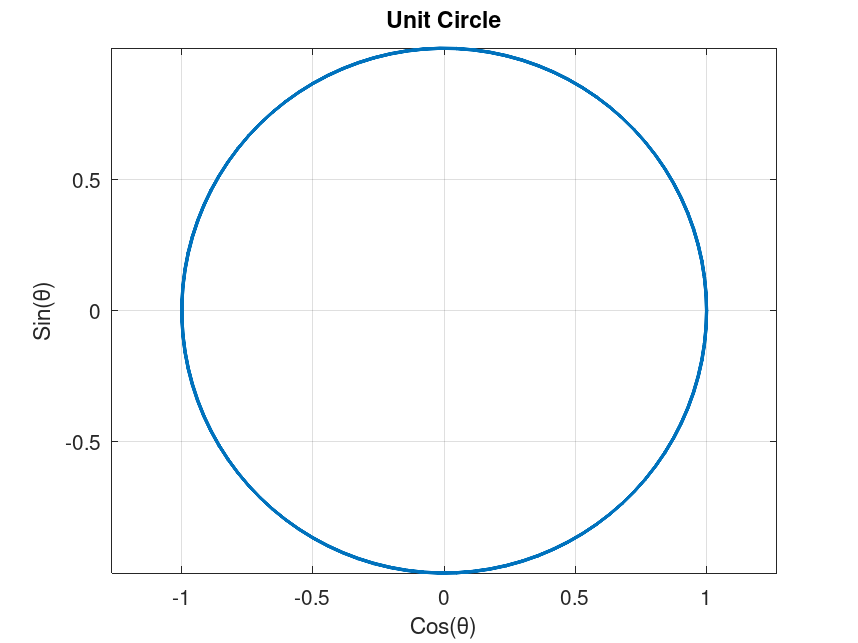
\includegraphics[width=0.5\linewidth]{unit-circle}
		\captionof{figure}{The Unit Circle}
		\label{fig:uc1}
	\end{center}

	\begin{color}{red}
	\textbf{Note:} Most graphing utilities like graphing calculators easily graph functions but require relationss to be broken into pieces for graphing.
	\\
	\emph{Example:} $y = \sqrt{1-x^2} and y=-\sqrt{1-x^2}$
	\end{color}


	\section{Intercepts}
	\begin{color}{blue}
		Intercepts are the points where a graph touches an axis.
		\\
		\emph{Example:} $y = 4x-8$ has
		\begin{tabular}{c c}
			x-intercept & (2,0)\\
			y-intercept & (0,-8)
		\end{tabular}
	\end{color}
	
	\section{Symmetries}
	\begin{itemize}
		\item A graph is symmetrical about the y-axis if (a,b) is on the graph whenever (-a,-b) is. 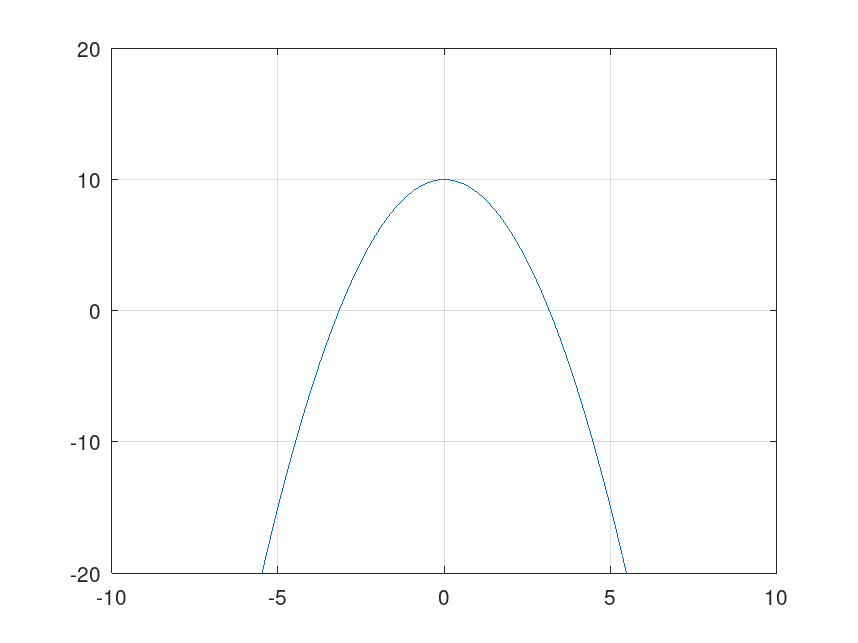
\includegraphics[width=0.2\linewidth]{basic-parab}
		\item A graph is symmetrical about the x-axis if (a,b) is on the graph whenever (a,-b) is. 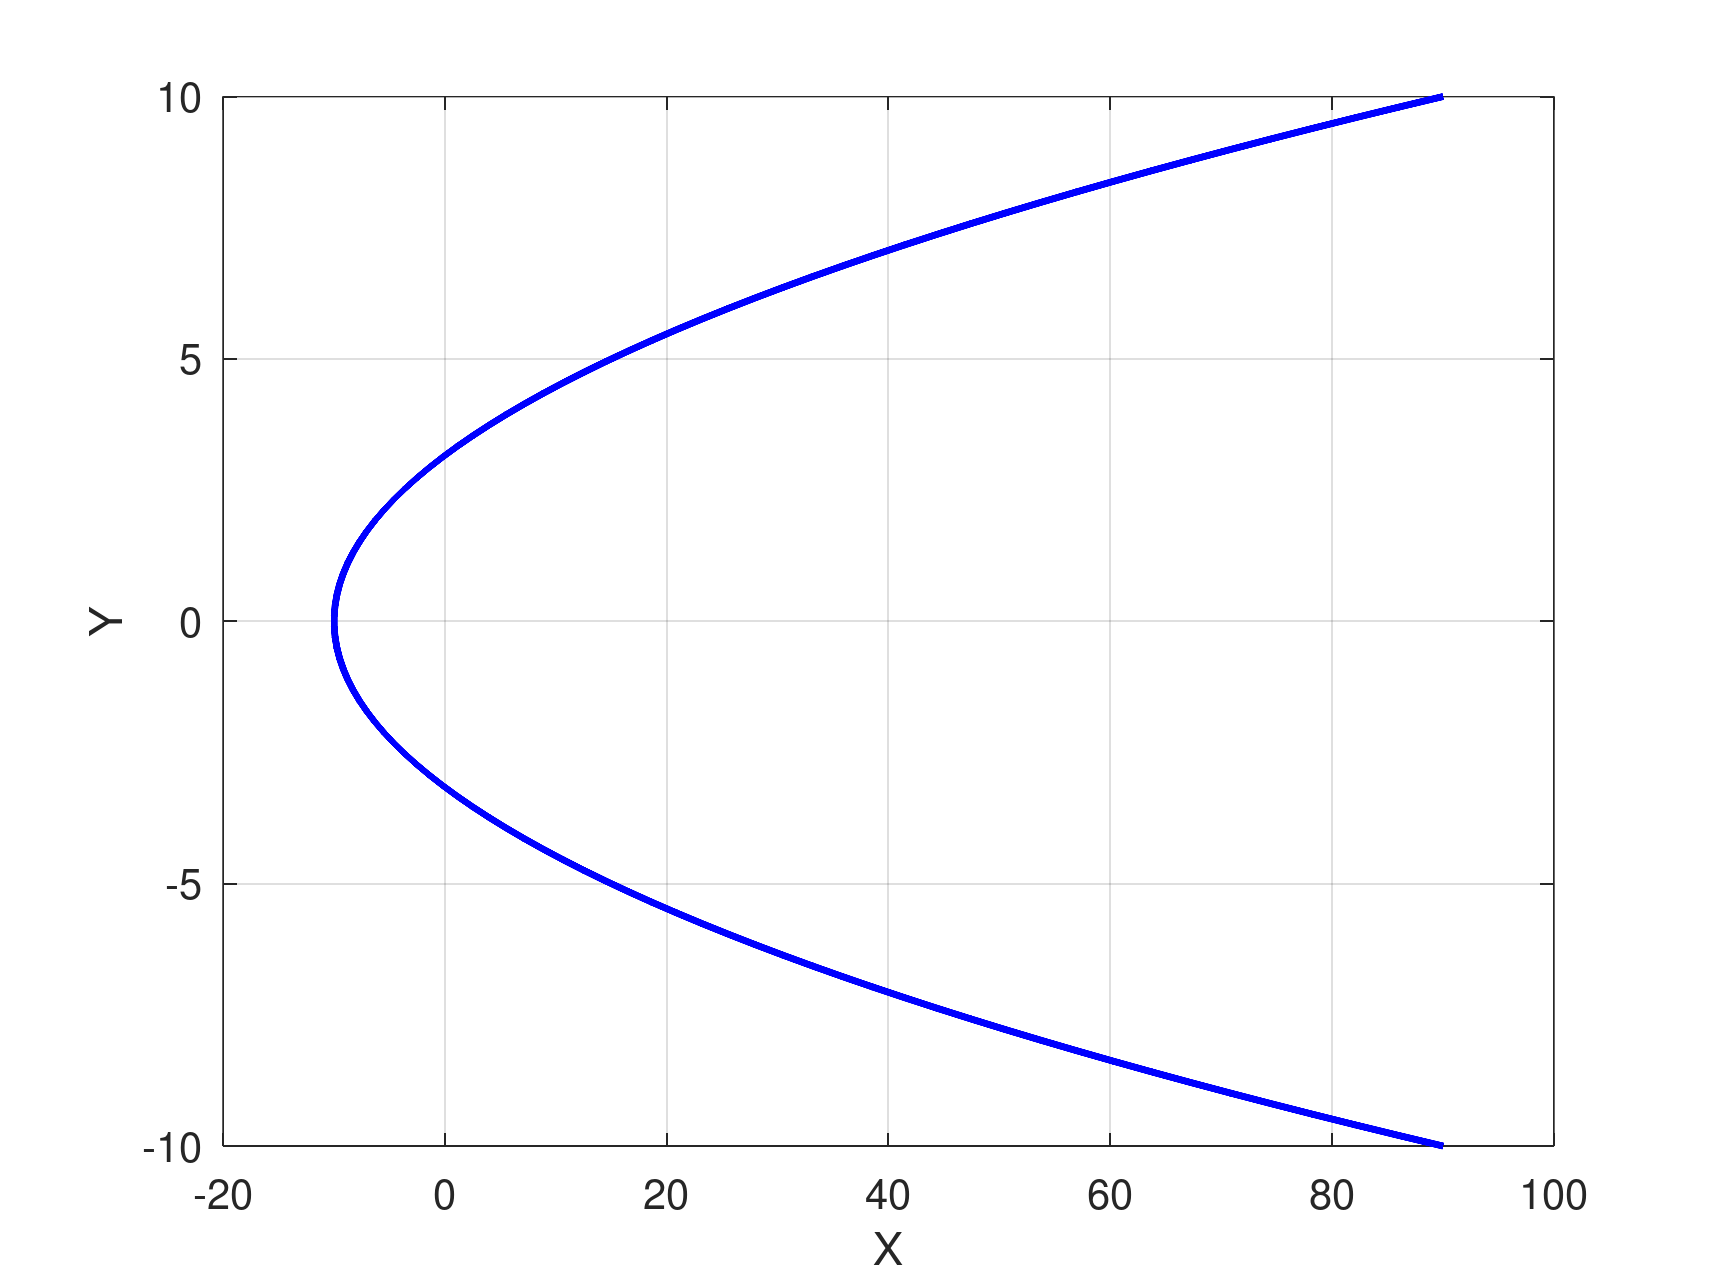
\includegraphics[width=0.2\linewidth]{vert-symmetry}
		\item A graph is symmetrical about the origin if (a,b) is on the graph whenever (-a,-b) is. 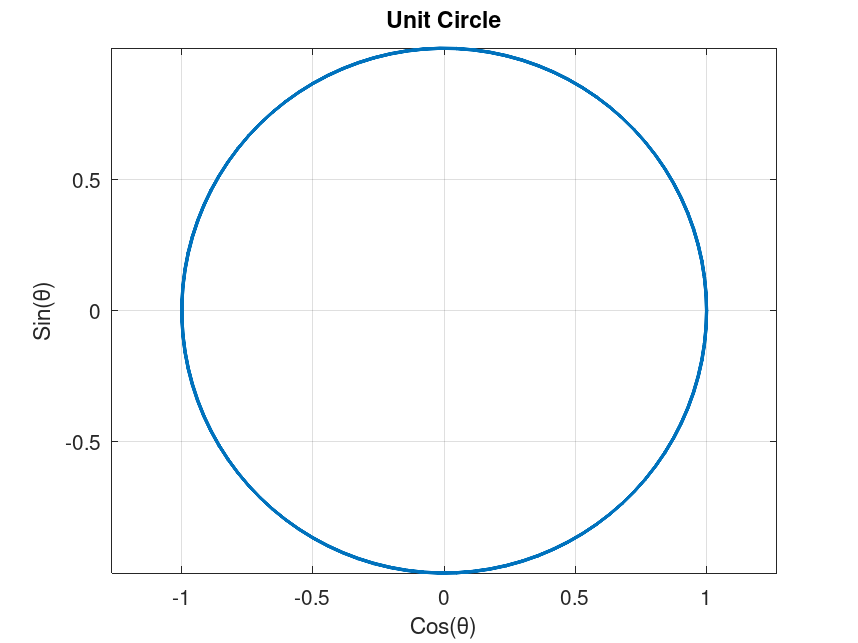
\includegraphics[width=0.2\linewidth]{unit-circle}
	\end{itemize}

	To test for symmetries, replace x with -x and y with -y in the equation of the graph and simplify.
	\\
	If the equation simplifies to the original form it has symmetry.
	\\

	\begin{tabular}{|c|c|c|}
		\hline
		x-axis & y-axis & origin
		\\
		\hline
		$x \leftrightarrow -x$ & $y \leftrightarrow -y$ & $x \leftrightarrow -x$
		\\
		& & $y \leftrightarrow -y$
		\\
		\hline
	\end{tabular}

	An intersection is a point where 2 graphs touch. It is found by solving the system of equations or using the graph.

	\begin{color}{red}
		A mathematical model is an equation or graph that represents a real world situation.
	\end{color}

	\pagebreak
	\section{Practical Problems}
	
	\#12 Sketch the graph by plotting points.
	
	\begin{center}
		$y=abs(2)-1$
	\end{center}
	
	\begin{tabular}{c|c|c}
		\hline
		X & f(x) & Y
		\\
		\hline
		-2 & $|-2|-1$ & 1
		\\
		-1 & $|-1|-1$ & 0
		\\
		0 & $|0|-1$ & -1
		\\
		1 & $|1|-1$ & 0
		\\
		2 & $|2|-1$ & 1
	\end{tabular}
	\\
	\#22. Find any intercepts
	\newline
	\begin{center}
		$y^2=x^2-4x$
	\end{center}
	\begin{multicols*}{2}
		x-intercepts: Set $y=0$
		\\
		$y^2 = x^2 - 4x$
		\\
		$0^2 = x^2 - 4x$
		\\
		$0 = x^2 - 4x$
		\\
		$0 = x(x-4)$
		\\
		$x=0 \Rightarrow (0,0)$
		\\
		$x-4=0 \Rightarrow (4,0)$
		\\

		\columnbreak
		y-intercepts: Set $x=0$
		\\
		$y^2 = x^2 - 4x$
		\\
		$y^2 = 0^2 - 4(0)$
		\\
		$y^2 = 0$
		\\
		$y=0 \Rightarrow (0,0)$
		\\
	\end{multicols*}
	#34 Test for Symmetry
	\\
	\begin{center}
		$xy^2=-10
	\end{center}

\end{document}